\documentclass[11pt,letterpaper]{article}     % Tipo de documento y otras especificaciones
\usepackage[utf8]{inputenc}                   % Para escribir tildes y eñes
\usepackage[spanish]{babel}                   % Para que los títulos de figuras, tablas y otros estén en español
\addto\captionsspanish{\renewcommand{\tablename}{Tabla}}					% Cambiar nombre a tablas
\addto\captionsspanish{\renewcommand{\listtablename}{Índice de tablas}}		% Cambiar nombre a lista de tablas
\usepackage{geometry}                         
\geometry{left=30mm,right=30mm,top=25mm,bottom=28mm} % Tamaño del área de escritura de la página
\usepackage{ucs}
\usepackage{amsmath}      % Los paquetes ams son desarrollados por la American Mathematical Society
\usepackage{amsfonts}     % y mejoran la escritura de fórmulas y símbolos matemáticos.
\usepackage{amssymb}
\usepackage{graphicx}     % Para insertar gráficas
%\usepackage{graphics}     % Para insertar gráficas
\usepackage[lofdepth,lotdepth]{subfig}	% Para colocar varias figuras
\usepackage{unitsdef}	  % Para la presentación correcta de unidades
\usepackage{pdfpages}   %incluir paginas de pdf externo, para los anexos
\usepackage{appendix}   %para los anexos
\renewcommand{\unitvaluesep}{\hspace*{4pt}}	% Redimensionamiento del espacio entre magnitud y unidad
\usepackage[colorlinks=true,urlcolor=blue,linkcolor=black,citecolor=black]{hyperref}     % Para insertar hipervínculos y marcadores
\usepackage{float}		% Para ubicar las tablas y figuras justo después del texto
\usepackage{booktabs}	% Para hacer tablas más estilizadas

\usepackage{tikz} %preamble
\usepackage{pgfplots}
\usetikzlibrary{decorations.pathmorphing}
\usepackage{tikz-3dplot}
\usepackage{listings}
\lstset{language=C++}

\usepackage{cleveref}
\usepackage{hyperref}

\batchmode
%\usepackage{apacite}
\bibliographystyle{plain} 
\pagestyle{plain} 
\pagenumbering{arabic}
\usepackage{lastpage}
\usepackage{fancyhdr}	% Para manejar los encabezados y pies de página
\pagestyle{fancy}		% Contenido de los encabezados y pies de pagina
%%%%%%%%%%%%%%%%%%%%%%%%%%%%%%%%%%%%%%%%%%%%%%%%%%%%%%%%%%%%%%%%%%%%%%%%%%%%%%%%%%%%%%%%%%%%%%%%%%%%%%%%%%%%%%%%%%%%%%%%%%%%%%%%%%%%%%%%%%%%%%%%%
%No modificar las líneas anteriores


\lhead{Investigación bibliográfica I}
\chead{}
\rhead{IE-0217 - Estructuras abstractas.}	% Aquí va el numero de experimento, al igual que en el titulo
\lfoot{Escuela de Ingeniería Eléctrica}
\cfoot{\thepage\ de \pageref{LastPage}}
\rfoot{Universidad de Costa Rica}

\author{Autor: \\ \\Jean Carlos Chavarría Hughes, B11814\\ \\ \\ \\ \\Profesor:\\ \\Dr. rer. nat. Francisco Siles Canales \vspace*{2.0in}}
\title{Universidad de Costa Rica\\{\small Escuela de Ingeniería eléctrica\\ IE-0217 - Estructuras abstractas de datos y algor\' itmos para ingeniería\\II ciclo 2014\\\vspace*{0.55in} Investigación bibliográfica I}\\ Formatos informáticos para objetos en 3D.
\vspace*{1.35in}}

%% Settings of tikz figures
\tikzset{isometricXYZ/.style={x={(-0.866cm,-0.5cm)}, y={(0.866cm,-0.5cm)}, z={(0cm,1cm)}}}
%: isometric South West : Z , South East : X , North : Y
\tikzset{isometricZXY/.style={x={(0.866cm,-0.5cm)}, y={(0cm,1cm)}, z={(-0.866cm,-0.5cm)}}}
%: isometric South West : Y , South East : Z , North : X
\tikzset{isometricYZX/.style={x={(0cm,1cm)}, y={(-0.866cm,-0.5cm)}, z={(0.866cm,-0.5cm)}}}


\begin{document}

\pdfbookmark[1]{Portada}{portada} 	% Marcador para el título

\maketitle
\newpage
\tableofcontents
\newpage
\listoffigures
\newpage

\section{Resumen}
En este proyecto se presentan y analizan diferentes tipos de estructuras de datos que se encuentran en la actualidad para el manejo de informaci\' on que representa objetos y figuras s\' olidas en tres dimesiones. Se busca presentar una discusi\' on de los formatos de archivos m\' as importantes, adem\' as, mostrar al lector los algoritmos m\' as importantes de manipulaci\' on de datos gr\' aficos y finalmente indagar sobre las cuatro representaciones de la malla poligonal, conocida en ingl\' es como \textit{polygonon mesh}.


\section{T\' itulo}
Estructuras de datos para gr\' aficos en tres dimensiones, con \' enfasis en algoritmos de comparaci\' on.

\section{Problema de la investigaci\' on}
La ausencia importante sobre descripciones sencillas que permitan implementar algoritmos de comparaci\' on de gr\' aficos en tres dimensiones, mediante la obtenci\' on y manipulaci\' on de archivos de texto que contengan vectores de posici\' on de diferentes indicadores en tiempo real. 

\section{Justificación}
La presente investigaci\' on se motiva debido a la creciente importancia que ha tomado la manipulaci\' on digital de informaci\' on en la actualidad, donde lograr predecir comportamientos y comparar actividades de ciertos objetos o personas con una referencia establecida no se ha podido llevar a cabo tan objetivamente como se quisiera. Por ejemplo en actividades deportivas, donde la presencia de jueces conlleva inherentemente agregar puntos de falla a la actividad debido a que como cualquier ser humano o conjunto de seres humanos, la percepci\' on e interpretaci\' on de im\' agenes debe pasar por la mente, donde cada persona puede tener perspectivas distintas, sin que exista un lineamiento completamente grande para abarcar cualquier eventualidad que se pueda presentar.\\
Existen muchas \' areas de la vida donde seria una ventaja lograr incorporar mecanismos de comparaci\' on de video, para determinar coincidencias, similitudes o divergencias entre cada uno de ellos, as\'i como generar bases estad\' isticas basadas no en datos num\' ericos, sino en la caracter\' istica de las acciones ejecutadas y digitalizadas.\\
Es por esta raz\' on que con la presente investigaci\' on se busca iniciar dicho proceso mediante el an\' alisis de estructuras de datos y algoritmos para obtener una base te\' orica suficientemente comprensible y aplicar el conociemiento a problemas gen\' ericos, de distintas \' indoles.


\section{Objetivos}
\subsection{Objetivo General}
Presentar una base te\' orica comprensible sobre estructuras de datos relacionadas con objetos en tres dimensiones, adem\' as de las cuatro representaciones de mallas poligonales.
\subsection{Objetivos Espec\' ificos} 
%Recuerde que se realiza un capitulo de investigacion por cada objetivo especifico. Sin perder de vista el objetivo general.
\begin{enumerate}
\item Comparar las caracter\' isticas de los formatos de gr\' aficos en tres dimensiones m\' as importantes que se manejan en la actualidad.
\item Presentar un an\' alisis de las siguientes tres representaciones de mallas poligonales:
	\begin{itemize}
	\item Mallas v\' ertice-v\' ertice.
	\item Mallas cara-v\' ertice.
	\item Mallas de bordes-alado.
%	\item Mallas de graficaci\' on din\' amica.
	\end{itemize}

%\item Brindar una descripci\' on detallada de los siguientes algoritmos: 
%	\begin{itemize}
%	\item Cierre transitivo.
%	\item Algoritmo de Warshall.
%	\item Algoritmo de trayectoria m\' as corta.
%	\item 
%	\end{itemize}
%

\item Describir los tipos de visualizaci\' on de conjuntos de datos:
	\begin{itemize}
	\item Representaci\' on de campos escalares.
	\item Representaci\' on de campos vectoriales.
	\item Representaci\' on de campos tensores.
	\end{itemize}
	
\end{enumerate}

\section{Introducci\' on}

Desde que surgieron los ordenadores, las tecnolog\' ias de la informaci\' on han cambiadado de manera tal que se puede considerar con un hito en la historia del ser humano. Desde ese momento, los avances en el \' area de las inform\' atica han crecido a pasos agigantados y en la actualidad el procesamiento de im\' agenes por computaci\' on y el an\' alisis de estas se ha convertido en un \' area de car\' acter cient\' ifico con gran importancia para la investigaci\' on e industria.\\
Los gr\' aficos son una estructura de datos, que permiten visualizar e interpretar informaci\' on de maneras muy llamativas al ser humano y con esto obtener tanto gr\' aficos en una dimensi\' on, dos dimensiones y tres dimensiones, por el momento.\\
Finalmente, este proyecto se presenta dentro de un marco en el cual la investigaci\' on dentro de la Escuela de Ingenier\' ia El\' ectrica ha crecido considerablemente, espec\' ificamente en el \' ambito de inteligencia artifical y reconocimiento de patrones, concibiendo de esta manera la necesidad de nichos de investigaci\' on centrados en temas espec\' ificos, como el presente.


\section{Desarrollo}
%%Capitulo 1
\subsection{Formatos de archivos}
En realidad existe un n\' umero extenso de tipos de archivos utilizados para la administraci\' on de objetos tridimensionales. En esta investigaci\' on se va a desarrollar un an\'  alisis de los cuatro tipos m\' as importantes para el \textit{MoCap}. Los cuales son:
\begin{itemize}
\item BVH.
\item C3D.
%\item CSV.
\item FBX.
\item POV.
\end{itemize}

\subsubsection{Formato C3D}
Este tipo de formato fue introducido con el objetivo de combatir el problema que existe entre los usuarios de sistemas de captura de movimiento y laboratorios biom\' edicos que tienen dificultades para compartir sus archivos con otros ya sea porque difieren del software utilzado o inclusive existen diferencias entre el mismo software pero diferentes versiones. 
El desarrollador principal de este formato fue el Doctor Andrew Dainis en 1987, a quien se le atribuye la primer versi\' on y quien consigui\' o aceptaci\' on en institutos nacionales de laboratorios de biomedicina en Bethesda, Maryland, adem\' as de muchos otros alrededor del mundo.  C3D tiene la capacidad de producir datos a partir de cualquier fabricante de dispositivos y cumple con las siguientes caracter\' isticas:
\begin{itemize}
\item Preserva informaci\' on que describe el tipo de dise\~ no f\' isico utilizado del laboratorio, tal como posiciones de platos, conjunto de marcas y tipos de canales empleados, EMG, entre otros.

\item Almacena informaci\' on relacionada con las circunstancias de la pr\' actica, tal como la raz\' on de muestreo, nombres de archivos, fechas, etc.

\item Alamacena informaci\' on del paciente como nombre, edad, peso, longitud de piernas, etc.

\end{itemize}

T\' ecnicamente el formato almacena coordenadas tridimensionales e informaci\' on num\' erica de cualquier tipo de medici\' on. La capacidad de almacenar m\' ultiple informaci\' on relacionada con los datos y la facilidad con que se pueden agregar m\' as datos a este tipo de archivos lo hacen muy llamativo.

Este formato se divide en dos secciones:

\begin{enumerate}
\item Cada coordenada 3D es almacenada como conjunto X,Y,Z con informaci\' on acerca de la muestra, presici\' on, error y m\' as informaci\' on que pueda aportar la c\' amara. 
Tambi\' en cada muestreo de datos num\' ericos contiene informaci\' on anal\' ongica tal como EMG y su interrelaci\' on con los vectores 3D. 

\item Informaci\' on param\' etrica. Adem\' as de las mediciones f\' isica, un fichero 3D de este formato contiene informaci\' on sobre unidades de medida, etiquetas de puntos, nombres de archivos y temas, diagnosticos y otros tipos de datos que se pueden utilizar en evaluaciones de protocolos posteriores.
\end{enumerate}

Finalmente se puede mencionar que al tener toda la informaci\' on en un solo fichero, se aumenta la confidencialidad de la informaci\' on, adem\' as que se obtiene una ventaja sobre los formatos OEM (Object Exchange Model) en tanto que en estos el video y la informaci\' on anal\' ogica se transfieren separadamente. Se puede recordar que un formato OEM es una o varias bases de datos orientadas a objetos. 

Algunas aplicaciones se pueden descargar en la direcci\' on: \href{url}{http://www.c3d.org/c3dapps.html}.

Para crear archivos en este formato se puede seguir el procedimiento descrito por \cite{c3d_pdf}, lo cual resumidamente se expresa en:
\begin{itemize}
\item La primer secci\' on que contiene el encabezado, es de 512 bytes y almacena cierta informaci\' on de par\' ametros.
\item La siguiente secci\' on comienza con una localizaci\' on indicada por el puntero en el encabezado y contiene los par\' ametroos almacenados en un \' unico formato. Su extensi\' on es variable, aproximandamente 10 bloques de longitud.
\item La tercer secci\' on comienza con una localizaci\' on indicada por un puntero en el encabezado y contiene los datos de coordenadas 3D, informaci\' on anal\' ogica si la hay y la conclusi\' on o fin del fichero.
\end{itemize}

Se puede observar una imagen ilustritiva en la Figura \ref{fig:c3d1}.

\begin{figure}[hbtp]
\caption{Uso en la biomedicina}
\centering
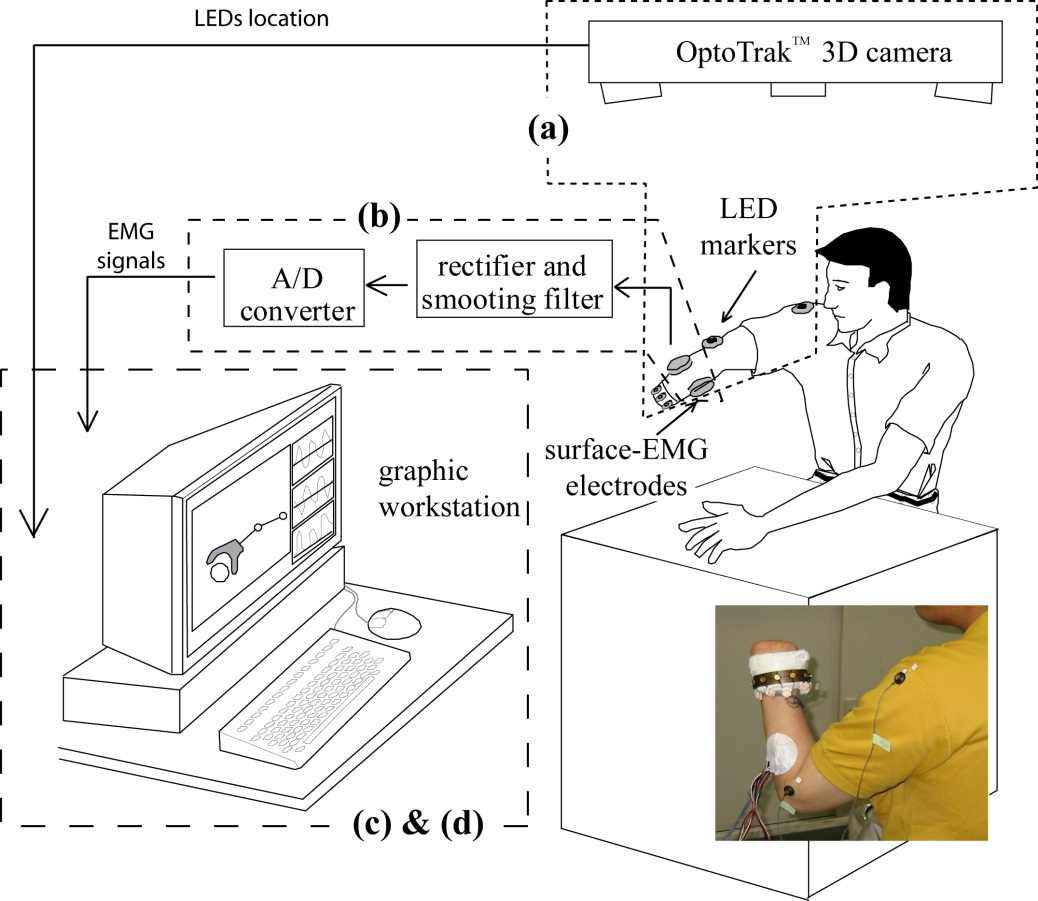
\includegraphics[scale=0.65]{imagenes/image22.jpeg}
\label{fig:c3d1}
\end{figure}

%\subsubsection{Formato CSV}
%Conocido en ingl\' es como el formato \textbf{comma separated values}, consiste en un documento de texto plano que contiene sequencias de caracteres sin ser interpretados como datos binarios. Cada grabaci\' on est\' a separada por brincos de linea  y todas las grabaciones tienen los campos id\' enticos.

\subsubsection{Formato BVH}
El formato BVH fue originalmente desarrollado por Biovision, una compa\~ nia que brinda servicios de captura de movimiento y significa en ingl\' es: Biovision hirarchical data. 

\paragraph{Aspectos t\' ecnicos.}
Un fichero de tipo BVH se compone de dos partes principales, el encabezado es denominado \textbf{HIERARCHY} contiene el inicio del \textbf{ROOT}. Despu\' es del ROOT se especif\' ica el segmento de jerarqu\' ia que va a ser definido. Existen ciertas reglas de sint\' axis como es costumbre, por ejemplo, que un TAB no puede ser sustituido por varios \textit{spaces}. 
Dentro de un ROOT se pueden definir varios segmentos, cada uno de los cuales debe contener con tres secciones:
\begin{itemize}
\item \textit{OFFSET}, el cual es especificado es coordenadas X,Y,Z. 
\item Luego se definen los \textit{CHANNELS}, la palabra reservasa para los canales, en donde se indica el n\' umero de estos y etiquetas para cada tipo de canal (en general el root debe mantener 6 canales y los subelementos del root 3 canales).
\item Finalmente se define ya sea un \textit{JOINT} o un \textit{End Site}. El primero es como un nuevo ROOT exepto por el n\' umero de canales. En cambio el End Site indica que el segmento actual esta en su final y no contin\' ua ning\' un otro elemento. \footnote{ver Ap\' endice  \nameref{Apendx:BHV}}.

Despu\' es del ROOT, se define la segunda parte del fichero, el \textbf{MOTION}, la cual es la secci\' on que contiene el n\' umero de \textit{frames}, el \textit{frame time} (el cual indica la raz\' on de muestreo de la informaci\' on, por ejemplo, un frame time de 0.0333 indica 30 frames por segundo), y el resto del fichero contiene la informaci\' on capturada de movimiento donde cada l\' inea es una muestra de movimiento y los n\' umeros aparecen en el orden de las especificaciones del canal tal como fue almacenado en la jerarqu\' ia del esqueleto.

\paragraph{Interpretaci\' on}
Para calcular la posici\' on de un segmento primero se crea una matriz de transformaci\' on que permita partir de la traslaci\' on y rotaci\' on local de cada segmento. 
Para la traslaci\' on se puede basar en el 
\textit{offset} de cada segmento, pero para la rotaci\' on se debe trabajar con la informaci\' on disponible en la secci\' on de movimiento.
El an\' alisis y la manipulaci\' on de estructuras de datos y ficheros que manejan posiciones en 3D y buscan la comparaci\' on de diferentes ficheros, asi como tambien la manipulaci\' on de dicha informaci\' on requiere una aplicaci\' on intensa de algebra lineal, en especial el manejo de espacios vectoriales y transformaci\' on de coordenadas \cite{BioVision}
\end{itemize}
Finalmente se puede obtener un visor de ficheros .BVH mediente el siguiente enlace, de manera gratuita.\\ \href{url}{http://vipbase.net/bvhviewer/}


\subsubsection{Formato FBX}
% direccion web http://en.wikipedia.org/wiki/FBX
% direccion web http://autodesk.typepad.com/bimtoolbox/2013/08/fbx-file-format-.html
Este tipo de archivo fue desarrollado por Kaydara y ahora administrado por Autodesk desde 2006 mas no se encuentra en su total madurez y para el 2011 todav\' ia se encontraba en fuertes investigaciones, lo cual indica que la informaci\' on disponible es poca. 
Igual que el tipo anterior, este busca almacenar la informaci\' on que se obtiene de dispositivos de captura de movimiento.
Una de las principales limitaciones de este tipo de formato no soporta el \textit{streaming} de datos y necesita enviar las escenas completas de manera continua, pero a\' un con tal limitante es un tipo de formato ppopular y usado por el software \textit{Cara.io}.

Con respecto a los aspectos t\' ecnicos, este formato es un poco similar al BVH en tanto que tiene dos secciones importantes en el fichero, el ROOT y los Hijos. Cada secci\' on comienza con un \textit{ObjectType} y luego se definen las propiedades en arreglos [] y como frases por lo que en t\' erminos de sint\' axis es muy diferente.

Se tiene objetos, los cuales son un conjuntos de varios tipos de elementos como luz, c\' amara, geometri\' ia, material, textura, etc y los cuales  se conectan unos con otros en la secci\' on de \textit{Connections}. 
Las conecciones son elementos de tipo C y poseen la siguiente informac\' on: 
\begin{itemize}
\item Define la naturaleza de la relaci\' on. Por ejemplo Objeto a Objeto u Objeto a Propiedad.
\item Dos UIDs, el primero es el hijo y el segundo es el padre en t\' erminos de jerarqu\' ia.
\end{itemize}

Y luego existen muchos otros datos que se pueden obtener como: \textit{Transformations constraints, spaces and parenting, light data, camera data, mesh data, null data, armature and bones, shape keys, material data, texture data and animation } \cite{fbxmanual}.

Finalmente se puede concluir que este formato esta especialmente dirigido a las aplicaciones de simulaci\' on de objetos y animaci\' on en 3D, debido a que trabaja con muchas propiedades que sirven para caracterizar los objetos f\' isicos pero en t\' erminos de movimiento no es muy \' agil. En la Figura \ref{fig:fbx1} se puede observar una imagen ilustrativa.

\begin{figure}[hbtp]
\caption{Ejemplo del uso de FBX}
\centering
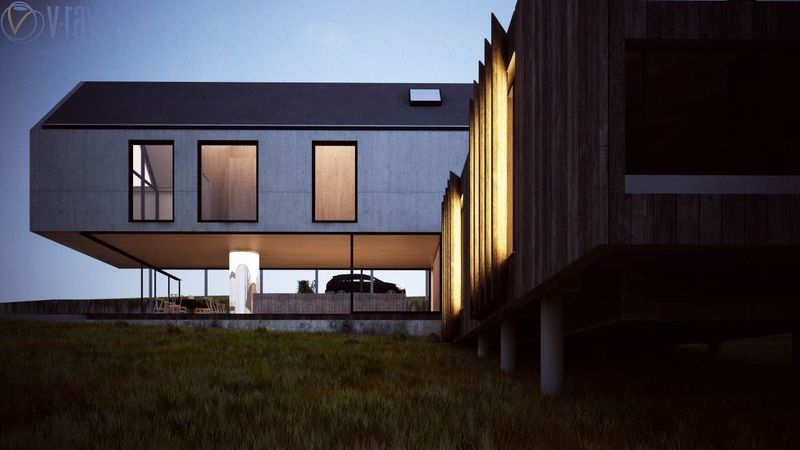
\includegraphics[scale=0.5]{imagenes/fbx1.jpg}
\label{fig:fbx1}
\end{figure}


\subsubsection{Formato POV}
Ya para el a\~ no 1993 este tipo de formato estaba desarrollado e implementado en ciertas aplicaciones por lo que se puede considerar uno de los m\' as maduros y basa principalmente en el efecto del \textit{Ray Tracing}, tal como se explica en el \footnote{ver Ap\' endice \nameref{Apendx:RayTr}}.

En t\' erminos generales es un tipo de lenguage de descripci\' on de escenas que se utiliza para representar imagenes de manera matem\' atica y utilizando efectos como la reflexi\' on, transparencia y luminosidad. Adem\' as, tiene la capacidad de crear imagenes muy realistas utilizando esta t\' ecnica y generar imagenes tipo TGA o GIF.

La informaci\' on almacenada en un POV es un conjunto de descriptores de escenas: c\' amaras, objetos y fuentes de luces. 

\begin{lstlisting}
//
// The canonical red ball on a green floor
//
camera {
	location <0 1 -2>
	look_at <0 1 2>
}
object {
	sphere { <0 1 2> 1 }
	texture { color red 1 phong 1 }
}
object {
	plane { <0 1 0> 0 }
	texture { color green 1 }
}
object {
	light_source { <3 3 -3> color red 1 green 1 blue 1 }
}
\end{lstlisting}

El anterior es un ejemplo donde se puede observar los tres elementos claramente identificados. 
Utiliza la sint\' axis muy similar al lenguage C standard o al C++ \cite{povformat}.

%\subsubsection{Formato SKP}
%http://en.wikipedia.org/wiki/SketchUp

%%Capitulo 2
\subsection{An\' alisis de mallas poligonales}
Cualquier tipo de modelado que se utilice, se basa en el desarrollo matem\' atico, lo  cual se conoce como modelo 3D (en el caso de s\' olidos). La representaci\' on puede llevarse a cabo mediante gr\' aficos en 2D con el proceso de \textbf{renderizado}, o en 3D mediante la simulaci\' on computarizada en un cinema f\' isico o una impresora especial.

Dicho tipo de representaci\' on se clasifica en dos categorias de acuerdo a la manera en que se realiza el modelado matem\' atico:

\begin{itemize}
\item Modelo s\' olido.Definición
El modelado s\' olido representa los objetos mediante su volumen, de esta manera se permite su manipulaci\' on no visual, pero es mucho m\' as complejo de modelar. Hay dos aplicaciones de este tipo de modelado: 

\begin{enumerate}
	\item Ray tracing. \footnote{ver Ap\' endice \nameref{Apendx:RayTr}}.
	\item Constructive solide geometry. \footnote{ver Ap\' endice \nameref{Apenx:CSG}}.
\end{enumerate}

\item Modelo superficial.
El modelo de supercifies cerradas no es tan realista como el anterior ya que no se basa en el volumen de la figura sino que emplea una copia del objeto por medio de l\' imites dados por pol\' igonos y segmentos.
Tambi\' en existe el modelado de superficies abiertas y es un caso simular al anterior en tanto que tampoco soportan la caracterizaci\' on del volumen ni momentos de inercia.
\end{itemize}
 
 En el presente documento se abarca el modelado en 3D utilizando superficies cerradas, esto debido a que el enfoque de la investigaci\' on busca realizar un modelado a partir de ciertas coordenadas conocidas en el espacio y tiempo.
 
\subsubsection{Malla de pol\' igonos}
Las superficies tridimensionales se pueden aproximar mediante un conjunto de pol\' igonos definidos adecuadamente e interpretados por alg\' un int\' erprete de estructura de datos, llamado malla de pol\' igonos.
Una malla de pol\' igonos define la forma de objetos tridimensionales representados por computadora mediante representaciones s\' olidas y se compone de l\' ineas, v\' ertices y caras (generalmente triangulares). Dado que esta representaci\' on es meramente geom\' etrica, se permite implementar operaciones sobre los objetos representados, tales como l\' ogica booleana, suavizado, simplificaci\' on entre otras.


\begin{itemize}
\item V\' ertices

Conocido como \textbf{vertex table}, contiene coordenadas en 3D de cada uno de los v\' ertices que conforman los pol\' igonos limitadores de la superficie. 
Puede contener informaci\' on como color, vector normal y textura.

\item Bordes

Contiene definiciones de la conexi\' on de cada borde en t\' erminos de \' indices de nodos y especif\' ica las conexiones de v\' ertices.

\item Caras

Se refiere a un conjunto cercano de bordes que conforman un pol\' igono establecido, generalmente un tri\' angulo pero tambien puede ser un cuadril\' atero u otro.
\end{itemize}
\subsubsection{Representaciones}
Las mallas de pol\' igonos se pueden representar es muchas maneras, depende de la manera en que se almacene la informaci\' on e inclusive es un \' area de investigaci\' on actual por lo que no se limita solo a los siguientes tipos.

\begin{itemize}
	\item Face-vertex.
	Este tipo representa a los objetos como un conjunto de caras y v\' ertices y t\' ipicamente es aceptado por los hardwards de procesamiento gr\' afico actual debido a su gran presici\' on y redimiento. De hecho es el m\' etodo m\' as empleado y se puede considerar como una mejora al Vertex-vertex ya que aqu\' i se brinda informaci\' on de manera expl\' icita sobre las caras alrededor de cada v\' ertice y sobre los v\' ertices que rodean cada cara, lo cual produce que la b\' usqueda de v\' ertices y caras tenga un tiempo constante, sin embargo, la b\' usqueda de bordes debe ser impl\' icita.
	\item Winged-edge.
	Este m\' etodo fue introducido por Baumgart en 1975 \cite{Baumgart} y es un avance sumamente importante en la calidad de representaci\' on de los objetos 3D. Provee informaci\' on sobre los tres elementos fundamentales de un objeto, caras, bordes y v\' ertices de manera expl\' icita, lo cual produce que los programas que lo utilicen posean mucha m\' as rapidez de procesamiento de la informaci\' on. Sin embargo no todo es bueno y en este caso su principal desventaja es que ncesita mucha m\' as capacidad de almacenamiento.
	
	\item Vertex-Vertex.
	Este tipo represeta a los objetos como un conjunto de v\' ertices conectados con otros v\' ertices y es la manera m\' as simple pero no la m\' as usada debido a que cuando se usa este tipo, la informaci\' on sobre las caras y los bordes del objeto se deben obtener de manera impl\' icita, lo cual significa m\' as procesamiento de informaci\' on. 
	Pero por otra parte, este tipo de representaci\' on tiene la ventaja de que utiliza muy poca cantidad de espacio para almacenar los datos de los objetos.
	
	\item Otros. Half-edge, quad-edge y  corner-tables.
	
\end{itemize}

%%Capitulo 3
\subsection{Tipos de visualizaci\' on de conjuntos de datos}
Los objetos en 3 dimensiones pueden ser representados de muchas maneras en aplicaciones gr\' aficas, algunas con limitantes y ventajas, pero en general todas se utilizan con el prop\' osito de representar lo mejor posible un objetivo. El uso  de m\' etodos gr\' aficos para el an\' alisis cient\' ifico se conoce por lo com\' un como \textbf{visualizaci\' on cient\' ifica} y permite simplificar la visualizaci\' on de procesos que de otra manera ocupar\' ian mucho tiempo y recursos. 
La visualizaci\' on cient\' ifica es un proceso de mapeo de las representaciones hechas por la computadora a representaciones precept\' uales, eligiendo t\' ecnicas de codificaci\' on para maximixar el entendimiento de comunicaci\' on con los seres humanos \cite{Tesis Americas Puebla Visualizacion}. B\' asicamente, la visualizaci\' on nos perminte interpretar datos que se obtienen de investigaciones matem\' aticas o cient\' ificas \cite{scottowen}, utiliza m\' etodos a partir de gr\' aficas por computadora, procesamiento de imagenes, visi\' on por computador y otras \' areas, para desplegar, resaltar y manipular informaci\' on a fin de permitir una mejor comprensi\' on \cite{Donald Hearn y M. Pauline Baker}.
Los tipos de datos se clasifican de acuerdo con su distribuci\' on e incluyen desde los unidimensionales como histogramas, bidimensionales como superficies hasta tridimensionales como espaciales.

\subsubsection{Representaci\' on visual de para campos escalares}
En general, un campo escalar es aqu\' el que se puede representar por medio de un solo valor como la distribuci\' on temporal, y adem\' as est\' an en funci\' on de otros par\' ametros escalares. Por ejemplo: densidad, masa, temperatura, presi\' on, carga, resistencia, entre otros.

M\' etodos comunes para visualizar campor escalares incluyen tablas, gr\' aficas de barras, de l\' inea, y adem\' as si los valores se encuentran distribuidos en una superficie se pueden emplear m\' etodos de interpolaci\' on para obtener gr\' aficas continuas
\cite{Donald Hearn y M. Pauline Baker}, como se puede observar en la Figura \ref{fig:scalarfield}.
Los m\' etodos de seudocolor tambi\' en se utilizan para distinguir diferentes valores en un conjunto de datos escalares y las t\' ecnicas de codificaci\'  on con colores un conjunto de datos escalares, elegimos un rango de colores y diagramamos el rango de valores de datos al rango de colores.
Los trazos de contorno se utilizan para desplegar isol\' ineas para un conjunto de datos que se distribuye en una superficie. Las isol\'  ineas est\'  an espaciadas en alg\'  un intervalo conveniente para mostrar el rango y la variaci\'  on de los valores de datos en la regi\'  on del espacio. Una aplicaci\'  on t\'  ipica es un trazo de contorno de elevaciones sobre un plano de terreno.
Para los campos de datos escalares tridimensionales, se puede tomar secciones de corte transversal y desplegar las distribuciones de datos bidimensionales en las secciones.  Finalmente para la presentaci\' on del volumen es otro m\' etodo para la visualizaci\'  on de conuntos de datos tridimensionales, pero profundizar en \' el se sale de los objetivos de la investigaci\' on propuestos.

\begin{figure}[hbtp]
\caption{Ejemplo de campo escalar}
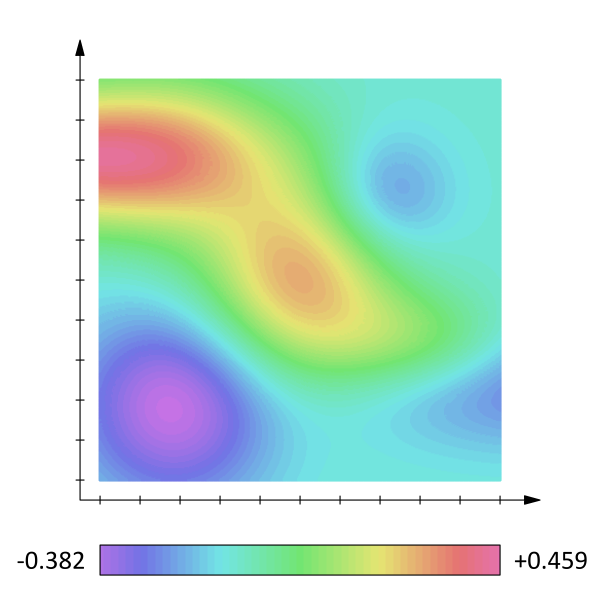
\includegraphics[scale=0.4]{imagenes/Scalar_field.png}
\label{fig:scalarfield}
\end{figure}


\subsubsection{Representaci\' on visual de para campos vectoriales}
Una cantidad vectorial \textbf{V} en un espacio tridimensional tiene tres valores escalares, \textit{Vx, Vy Yz}, uno para cada direcci\'  on de coordenada y un vector bidimensinal tiene dos componentes, \textit{Vx Vy}. Otra forma para describir una cantidad vectorial es al dar su magnitud y su direcci\'  on como un vector unitario. Al igual  que con los escalares, las cantidades vectoriales pueden ser funciones de posici\'  on, tiempo y otros par\' ametros. Una manera para visualizar un campo vectorial es trazar cada punto de datos como una peque\~ na flecha que indica la magnitud y direcci\'  on del vector.
Las magnitudes para los valores vectoriales se pueden mostrar al variar las longitudes de las flechas o modificar los colores de acuerdo a un c\'  odigo establido. Tambi\'  en se pueden representar valores vectoriales con l\'  ineas de flujo o l\'  ineas de campo, tal y como se puede observar en la Figura \ref{tikz:campovectorial} \cite{Donald Hearn y M. Pauline Baker}.

\begin{figure}
\begin{tikzpicture}
\def \angle{pi/8}
\pgfmathsetmacro{\dang}{deg(\angle)}
\draw (0, 0) grid (4, 3);

\foreach \x/\k in {0.5/1, 1.5/2, 2.5/3, 3.5/4} {
  \foreach \y in {0.5, 1.5, 2.5} {
      \fill (\x,\y) circle[radius=1pt];
     %  \draw[->,thick]  (\x, \y) -- ++(\k*\dang:1);
	 \draw [thick] (\x,\y) --++(\k*\dang:1);
    }
}

\end{tikzpicture}
\caption{Ejemplo de un campo vectorial} 
\label{tikz:campovectorial}
\end{figure}



\subsubsection{Representaci\' on visual de para tensores}
Una cantidad tensora en un espacio tridimensianl tiene nueve componentes y se puede representar con una matriz de 3 por 3. En realidad, esta representaci\'  on se utiliza para un tensor de segundo orden y los tensores de orden mayor ocurren en algunas aplicaciones como la relatividad general.
Las cantidades de tensor se encuentran con frecuencia en los materiales anisotr\'  opicos, que tienen diferentes propiedades en distintas direcciones. 
En lugar de intentar visualizar los seis componentes de una cantidad tensorial, podemos reducir el tensor a un vector o a un valor escalar al utilizar una representaci\'  on vectorial, se puede desplegar simplementar para los elementos diagonales de tensor, y para obtener representaciones escalares se pueden usar operaciones de contracci\'  on. Como se puede observar en la Figura \ref{fig:tensorfield} \cite{Avizo Standard} \cite{Donald Hearn y M. Pauline Baker}.

\begin{figure}[hbtp]
\caption{Ejemplo de Campo tensorial}
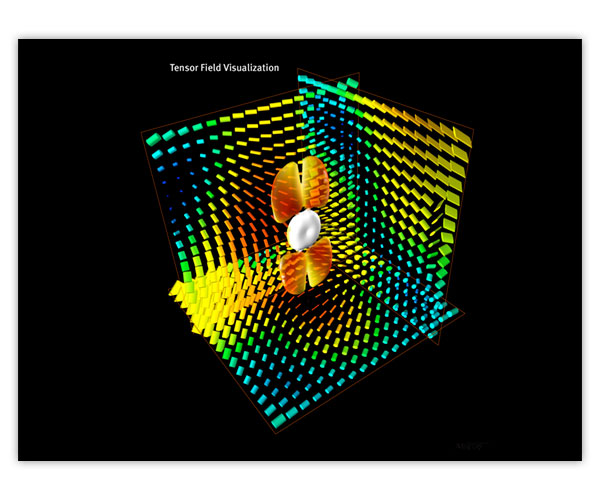
\includegraphics[scale=0.6]{imagenes/AvizoStandard_Tensor_field_visualization.jpg}
\label{fig:tensorfield}
\end{figure}

%\begin{figure}[hbtp]
%	\centering	
%	\caption{Realistic Ray Tracing}
%	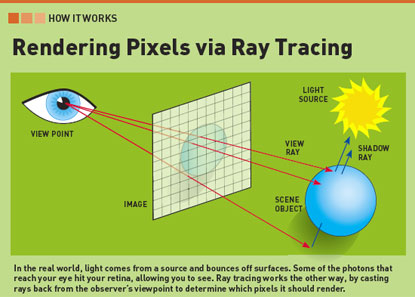
\includegraphics[scale=0.6{./imagenes/realistic_raytracinglarge.png}
%	\label{fig:ray1}
%\end{figure}

\begin{figure}
	\centering
		\includegraphics[scale=0.5]{./imagenes/renderingpixels.jpg}
	\caption{Ejemplo de ray tracing \cite{raytr}}
	\label{fig:ray2}
\end{figure}




\section{Conclusiones}

\appendix
\section{Ray tracing}\label{Apendx:RayTr}
El \textit{ray tracing}, o trazado de rayos es una t\' ecnica que permite calcular imagenes de escenas mediante la simulaci\' on de los rayos de luz que atraviesan es espacio. Sin embargo, se puede recordar que en el mundo real, los rayos de luz se emites de fuentes luminosas e ilumnia objetos, se refleja en objetos y atravisa objetos transparentes. Este rayo reflejado impacta sobre espectadores, como por ejemplo un lente de c\'  amara, es por esta raz\' on que una gran cantidad de rayos nunca llegan a ser observados.

Con esta t\' ecnica se especifica una posici\'  on para la c\'  amara o el observador en general, las fuente
de luz, los objetos tantos en forma con en textura y el ambiente que los rodea. En cada momento que un rayo impacta y se refleja sobre un objeto, se calcula tanto su intensidad como su \' angulo de reflexi\'  on \cite{RayTracing}. Algunos ejemplos se pueden observar en las Figuras \ref{fig:ray1} y \ref{fig:ray2}.


\begin{verbatim}{Algoritmo de Ray Tracing}
Para cada pixel de la imagen {
 Crear un rayo desde el punto de visión a través del pixelActual
 Inicializar NearestT al INFINITO y NearestObject a NULL
 Para cada objeto de la escena {
   Si el rayo se interseca con el objetoActual{
     Si t de la intersección es menor que NearestT {
         Poner NearestT = t de la intersección
         Poner NearestObject a objetoActual
     }
   }
 }
 Si NearestObject = NULL{
    Rellenamos pixelActual con el color de fondo
 }
 Sino{
    Lanzar un rayo a cada foco de luz para comprobar las sombras
    Si la superficie es reflectiva, generar un rayo reflectivo (recursivo)
    Si la superficie es transparente, generar un rayo refractante (recursivo)
    Usar NearestObject y NearestT para computar la función de sombreado
    Rellenar este pixel con el color resultante de la función de sombreado
 }
}
\end{verbatim}


\section{Constructive solid geometry}\label{Apenx:CSG}
La geometr\' ia de construcci\' on de s\' olidos es un tipo de geometria inteligente que provee informaci\' on extra mediante el uso de objetos simples llamados s\' olidos, construidos de acuerdo con ciertas reglas geom\' etricas. \cite{CSG pdf}
La caracter\' istica m\' as importante del CSG es que permite operaciones matem\' aticas que no son permitidas con mallas de pol\' igonos.
Hay muchas operaciones, pero para mencionar las dos m\' as b\' asicas:
\begin{itemize}
\item Ecuaci\' on de la distancia entre un punto y un plano. 
\item Ecuaci\' on de la intersecc\' on entre un rayo o recta y un plano.
\end{itemize}
Se puede observar en la Figura \ref{fig:csg1} y \ref{fig:csg2}, ejemplos donde se utiliza este mecanismo.

\begin{figure}
	\centering
		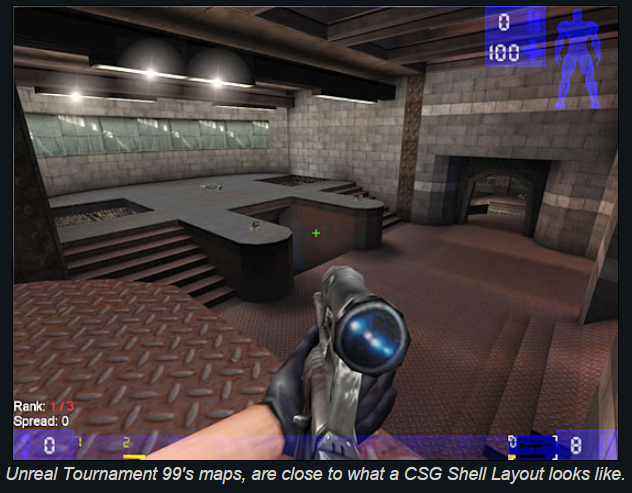
\includegraphics[scale=0.6]{./imagenes/unrealCSG.png}
	\caption{Unreal Tournament Graphics}
	\label{fig:csg1}
\end{figure}

\begin{figure}
	\centering
		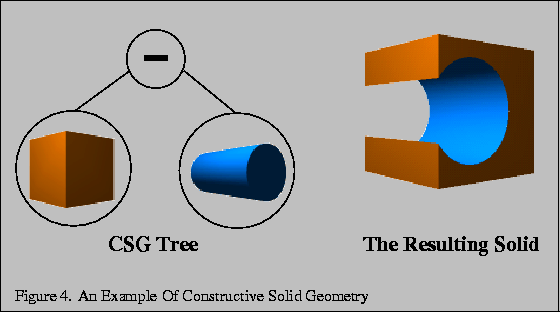
\includegraphics[scale=0.6]{./imagenes/csg.png}
	\caption{CSG example}
	\label{fig:csg2}
\end{figure}

\section{Ejemplo .BVH}\label{Apendx:BHV}
Se puede observar un ejemplo b\' asico de un fichero en .BVH mediante el siguiente link.\\ \href{url}{http://research.cs.wisc.edu/graphics/Courses/cs-838-1999/Jeff/Example1.bvh}.

Y en este otro enlace se puede observar un fichero m\' as avanzado con muchos m\' as frames.\\ \href{url}{http://vipbase.net/bvhviewer/01.bvh}.

Finalmente se puede realizar una b\' usqueda de aplicaciones para diferentes plataformas que permitan la lectura de este tipo de archivos en el siguiente enlace.\\ \href{url}{http://www.cs.man.ac.uk/~toby/bvh/}.


\newpage
\renewcommand{\bibname}{Referencias}
\addcontentsline{toc}{section}{Referencias}

\begin{thebibliography}{5}
\bibitem {G. Scott Owen} G. Scott Owen (2005). \textit{HyperGraph} Obtenido de \url{https://www.siggraph.org/education/materials/HyperGraph/hypergraph.htm}  el 1 de setiembre de 2014.

\bibitem {Langasam, Augenstein y Tenenbaum} Yedidyah Langasam, Moshe J. Augenstein y Aaron M. Tenenbaum (1997). \textit{Estructuras de datos con C y C++, Segunda Edicion}. Prentice Hall/Booklyn College, México D.F., México.

\bibitem {Donald Hearn y M. Pauline Baker} Donald Hearn y M. Pauline Baker (1995). \textit{Gr\' aficas por computadora, Segunda Edicion}. Prentice Hall/Hispanoamericana, México D.F., México.

\bibitem {Colin Smith} Colin Smith (2006). \textit{On Verrtex-Vertex systems and their use in geometric and biological modelling}. The University of Calgary/Departament of computer science, Calgary, Alberta.

\bibitem {Md Shonel, Leow Meng Chew y Pang Ying Han} Md Shonel, Leow Meng Chew y Pang Ying Han (2014). \textit{Computer Graphics, TCS2111}. Recuperado de \url{http://fist2.mmu.edu.my/} el 1 de setiembre de 2014.

\bibitem {Avizo Standard} Avizo® Standard, The 3D Analysis Software for Scientific Visualization. \textit{Avizo® Standard} Obtenido de \url{http://www.vsg3d.com/avizo/standard} el 19 de setiembre de 2014.

\bibitem {Baumgart} Bruce G. Baumgart, Stanford University. \textit{Winged-Edge Polyhedron Representation for Computer Vision}
Recuperado de \url{http://www.baumgart.org/winged-edge/winged-edge.html} el 21 de setiembre de 2014.

\bibitem {scottowen} Scott Owen, 24 de Octubre de 1999. \textit{Definitions, History, and Goals of Visualization.} Recuperado de \url{http://www.siggraph.org/education/materials/HyperVis/visgoals/visgoal0.htm} el 21 de setiembre de 2014.

\bibitem {Tesis Americas Puebla Visualizacion} Tesis de Licenciatura, Su\' arez Rold\' an, P. K. 2003. \textit{Animaci\' on y Visualizaci\' on de Fen\' omenos Naturales}. Recuperado de  \url{http://catarina.udlap.mx/u_dl_a/tales/documentos/lis/suarez_r_pk/indice.html} el 21 de setiembre de 2014.

\bibitem {CSG pdf} Constructive solid geometry, Copyright Leadwerks Corporation 2006. \textit{What is constructive solid geometry} Recuperado de \url{http://www.leadwerks.com/files/csg.pdf} el 21 de setiembre de 2014.

\bibitem {c3d_pdf} Motion Lab Systems. \textit{User Guide} Recuperado de \url{http://www.c3d.org/pdf/c3dformat_ug.pdf} el 24 de setiembre de 2014.

\bibitem {RayTracing} Persistence of Vision Raytracer Pty. Ltd. Copyright 2008. \textit{What is Ray-Tracing} Recuperado de \url{http://www.povray.org/documentation/view/3.6.2/4/} el 21 de setiembre de 2014.


\bibitem {raytr} University of UTAH \textit{ Realistic Ray Tracing} Recuperado de \url{http://www.cs.utah.edu/~wmartin/pics/rtrt/} el 21 de setiembre de 2014.

\bibitem {c3d} C3D.ORG \textit{The biomechanics standard} Recuperado de \url{http://www.c3d.org/sampledata.html} el 24 de setiembre de 2014.

\bibitem {BioVision} BioVision BVH. Micheal Gleicher  \textit{CS838 - Topics in Computer Animation. Wisconsin Madison} Recuperado de \url{http://research.cs.wisc.edu/graphics/Courses/cs-838-1999/Jeff/BVH.html} el 24 de setiembre de 2014.

\bibitem {fbxmanual} FBX File Structure  \textit{Blender Wiki} Recuperado de \url{http://wiki.blender.org/index.php/User:Mont29/Foundation/FBX_File_Structure} el 25 de setiembre de 2014.

\bibitem {povformat} POV format  \textit{POV File Format Summary
	} Recuperado de \url{http://www.fileformat.info/format/pov/egff.htm} el 25 de setiembre de 2014.

\end{thebibliography} 
\end{document}